% Typical processing for PostScript (PS) output:
%
%  latex advanced_example
%  bibtex advanced_example  (bibliography)
%  makeindex -s nomencl.ist -o advanced_example.gls advanced_example.glo
%                            (nomenclature)
%  latex advanced_example   (repeat as needed to resolve references)
%
%  xdvi advanced_example    (onscreen draft display)
%  dvips advanced_example   (postscript)
%  gv advanced_example.ps   (onscreen display)
%  lpr advanced_example.ps  (hardcopy)
%
% With the above, only Encapsulated PostScript (EPS) images can be used.
%
% Typical processing for Portable Document Format (PDF) output:
%
%  pdflatex advanced_example
%  bibtex advanced_example    (bibliography)
%  makeindex -s nomencl.ist -o advanced_example.gls advanced_example.glo
%                              (nomenclature)
%  pdflatex advanced_example  (repeat as needed to resolve references)
%
%  acroread advanced_example.pdf  (onscreen display)
%
% If you have EPS figures, you will need to use the epstopdf script
% to convert them to PDF because PDF is a limmited subset of EPS.
% pdflatex accepts a variety of other image formats such as JPG, TIFF,
% PNG, and so forth -- check the documentation for your version.
%
% If you do *not* specify suffixes when using the graphicx package's
% \includegraphics command, latex and pdflatex will automatically select
% the appropriate figure format from those available.  This allows you
% to produce PS and PDF output from the same LaTeX source file.
%
% To generate a large format (e.g., 11"x17") PostScript copy for editing
% purposes, use
%
%  dvips -x 1467 -O -0.65in,0.85in -t tabloid advanced_example
%
% For further details and support, read the Users Manual, aiaa.pdf.



\documentclass[]{aiaa-tc}% insert '[draft]' option to show overfull boxes

 \usepackage{varioref}%  smart page, figure, table, and equation referencing
 \usepackage{wrapfig}%   wrap figures/tables in text (i.e., Di Vinci style)
 \usepackage{threeparttable}% tables with footnotes
 \usepackage{dcolumn}%   decimal-aligned tabular math columns
  \newcolumntype{d}{D{.}{.}{-1}}
 \usepackage{nomencl}%   nomenclature generation via makeindex
  \makeglossary
 \usepackage{subfigure}% subcaptions for subfigures
 \usepackage{subfigmat}% matrices of similar subfigures, aka small mulitples
 \usepackage{fancyvrb}%  extended verbatim environments
  \fvset{fontsize=\footnotesize,xleftmargin=2em}
 \usepackage{lettrine}%  dropped capital letter at beginning of paragraph
 \usepackage[dvips]{dropping}% alternative dropped capital package
 \usepackage[colorlinks]{hyperref}%  hyperlinks [must be loaded after dropping]


%%%%% Title %%%%%
 \title{Multi-species Fluid Flow Simulations using a Hybrid Computational Fluid Dynamics - Molecular Dynamics Appraoch 
 \skonote{Or "Polyatomic Lagrangian Dynamics Modelling for a Hybrid Computational Fluid Dynamics - Molecular Dynamics Appraoch"} }
%%%%% End Title %%%%%


%%%%% Author %%%%%
 \author{
  Nayong Kim\thanks{A Post-doctoral Researcher; Center for Computation \& Technology,
  Louisiana State University, Baton Rouge, LA 70803, USA; Non-AIAA Member}\\
  {\normalsize\itshape
   Louisiana State University, Baton Rouge, LA 70803, USA}\\
  \and
  Soon-Heum Ko\thanks{A Computational Scientist; National Supercomputing Centre,
  Link\"{o}ping University, Link\"{o}ping, 581 83 Sweden; Non-AIAA Member}\\
  {\normalsize\itshape
   Link\"{o}ping University, Link\"{o}ping, 581 83, Sweden}\\
  \and
  Shantenu Jha\thanks{An Assistant Professor; Department of Electrical and Computer Engineering,
  94 Brett Road, Piscataway, NJ 08854, USA; Non-AIAA Member}\\
  {\normalsize\itshape
   Rutgers University, Piscataway, NJ 08854, USA}\\
  \and
  Dorel Moldovan\thanks{An Associate Professor; Department of Mechanical Engineering,
  Louisiana State University, Baton Rouge, LA 70803, USA; Non-AIAA Member}
    \ and
  Dimitris E. Nikitopoulos\thanks{A Professor; Department of Mechanical Engineering,
  Louisiana State University, Baton Rouge, LA 70803, USA; AIAA Member}\\
  {\normalsize\itshape
   Louisiana State University, Baton Rouge, LA 70803, USA}\\
 }
%%%%% End Author %%%%%


 % Data used by 'handcarry' option
 \AIAApapernumber{YEAR-NUMBER}
 \AIAAconference{Conference Name, Date, and Location}
 \AIAAcopyright{\AIAAcopyrightD{YEAR}}

 % Define commands to assure consistent treatment throughout document
 \newcommand{\eqnref}[1]{(\ref{#1})}
 \newcommand{\class}[1]{\texttt{#1}}
 \newcommand{\package}[1]{\texttt{#1}}
 \newcommand{\file}[1]{\texttt{#1}}
 \newcommand{\BibTeX}{\textsc{Bib}\TeX}


%%%%% Note Configuration %%%%%
\newcommand{\jhanote}[1]{ {\textcolor{red} { ***Jha: #1 }}}
\newcommand{\Nkimnote}[1]{ {\textcolor{blue} { ***NKim: #1 }}}
\newcommand{\skonote}[1]{ {\textcolor{green} { ***Jeff: #1 }}}
\newcommand{\menote}[1]{ {\textcolor{purple} { ***Comment from ME: #1 }}} 
%%%%% End Note Configuration %%%%%


\begin{document}

\maketitle


%%%%% Abstract %%%%%
\begin{abstract}
\skonote{Before going further, check the AIAA membership on co-authors: basically Dimitris is most likely to own the membership}
The constrained Lagrangian dynamics modelling in the hybrid computational fluid dynamics (CFD) - molecular dynamics (MD) approach is improved for the simulation of multi-species polyatomic fluid.
Microscopic mean velocity term on the classical Lagrangian dynamics equation is replaced by the division of mean linear momentum and mean mass to account for multi-species fluid system.
Also, the equation is applied on molecules instead of individual atom, to preserve the linear momentum between continuum and particle domain without encountering the unfaborable numerical break-down of molecular structure.
We verify our hybrid CFD-MD simulation package by analyzing a nano-scale transient Couette flow of a single monatomic fluid.
We will evaluate the multi-species polyatomic Lagrangian dynamics modelling by analyzing two different fluid models: the mixture of two monatomic fluids and a polyatomic molecular fluid under the short-range potential.
These two applications will describe the effect of particle-level mass variation on the macroscopic flow evolution.
\end{abstract}
%%%%% End Abstract %%%%%


%\printglossary %creates nomenclature section produced by MakeIndex


%%%%% Introduction %%%%%
\section{Introduction}
\label{sec:intro}

\lettrine[nindent=0pt]{T}{he} hybrid computational fluid dynamics (CFD) - 
molecular dynamics (MD) approach is getting more attraction as a potential 
answer in describing the nano-scale flow phenomena. In this approach,
the fluid system is divided into subdomains and individual subdomain is
solved by either the continuum solver or the particle-based solver.
Conventionally, the macroscopic flow region where the continuum hypothesis is
valid is resolved by the continuum formulation and the material interface 
(e.g. fluid/solid or fluid/fluid) is analyzed by higher degree-of-freedom 
particle formulation. Compared with the classical CFD or MD methodology, 
this approach is expected to provide the high-resolution solution near 
the wall boundary within the acceptable computational cost.

A number of scientific studies have been published which improve the hybrid
technique and/or apply this approach to various nano-scale flow fields.
These researches can be categorized to constrained Lagrangian dynamics
\cite{Thompson,Nie,Nie_cavity,Cui,Wang,Yen,Liu,JoCS2012}, alternating 
Schwarz method\cite{Hadjicon1,Hadjicon2,Hadjicon3,Werder,Kotsalis}, 
and direct flux exchange\cite{Flekkoy,Wagner,Delgado1,USHER,Time_Mechanism,Giupponi},
according to the formulation of hybrid shcemes and the characteristics of 
variables exchanged in the overlapping region. Of these methods, the 
constrained Lagrangian dynamics applies the constrained Lagrangian dynamics
equation to impose the hybrid MD boundary condition. Continuum and particle
solvers exchange density properties (i.e., conservative variables) 
and they are coupled in time space. Compared to other counterparts, this
method is easy to implement, is directly applicable to the unsteady flow 
simulation, and its molecular samples are less noisy than the flux properties.


%\lettrine[nindent=0pt]{T}{he} hybrid computational fluid dynamics (CFD) - 
%molecular dynamics (MD) approach is getting more attraction as a potential 
%answer in accurately describing the nano-scale flow phenomena within 
%the acceptable computational cost. A number of scientific studies have been
%published using this approach, which can be categorized to constrained 
%Lagrangian dynamics~\cite{Thompson,Nie,Nie_cavity,Cui,Wang,Yen,Liu,AJK2011}, 
%alternating Schwarz method~\cite{Hadjicon1,Hadjicon2,Hadjicon3,Werder,Kotsalis}, 
%and direct flux exchange~\cite{Flekkoy,Wagner,Delgado1,USHER,Time_Mechanism,Giupponi}.
%Of these methods, the constrained Lagrangian dynamics is easy to implement, 
%is directly applicable to the unsteady flow simulation, and molecular sample is
%less noisy than the flux-based approach.


Meanwhile, this approach is only valid for the single-species monatomic fluid 
flow since the constrained Lagrangian dynamics equation does not consider
the mass variation of fluid particles. So, the direct aplication of the classical
constrained Lagrangian dynamics equation to multi-species fluid domain results in
the break-up of momentum conservation. Also, the application to the polyatomic fluid
whose atomic mass are different ends up with the numerical break-up of chemical bond.

This motivates us to refine the classical constrained Lagrangian dynamics equation
for the application to multi-species and polyatomic fluid flow. The equation is
reformulated to provide the linear momentum conservation. Also, the equation is
applied on the molecules instead of individual atoms, to prevent the numerical
break-up of chemical bond. We implement this equation on our hybrid CFD-MD simulation
package which has been introduced in our previous article\cite{JoCS2012} and apply
it to solving multi-species and polyatomic fluid flow.

We introduce the hybrid CFD-MD approach and describe the Lagrangian dynamics equation
for multi-species polyatomic fluid particles in Section~\ref{sec:hybrid}. Numerical
methods and hybrid interface on individual solver will be addressed in Section
\ref{sec:numerics}. Section~\ref{sec:result} will be dedicated to present 
numerical solutions of the transient Couette flow in different fluid systems.
The first system consists of two monatomic fluids whose chemical properties are
equivalent to the liquid argon with the variation in mass. The next one contains
the polyatomic molecules whose molecular structure is equivalent to water while
the long-range interaction (i.e., Coulombic force) is not considered. We will 
summarize our studies and propose further applications in Section~\ref{sec:conclusion}.
%%%%% End Introduction %%%%%


%%%%% Hybrid Schema %%%%%
\section{Hybrid CFD-MD Approach for Multi-species Polyatomic Fluid}
\label{sec:hybrid}

\subsection{The Hybrid CFD-MD Approach}
\label{sec:hybrid_design}


A detailed structure of the fluid domain for the hybrid CFD-MD approach is
described in Figure~\ref{Fig:Couette}. CFD solves the flow region where 
the continuum hypothesis is valid while MD analyzes the complex microscopic 
flow feature near the solid obstacle. Overlapping region is placed sufficiently 
far from the solid stationary wall to prevent the direct influence of 
molecular-level physics.


%%%%% FIGURE %%%%%
%\begin{wrapfigure}{R}{0.6\linewidth}
%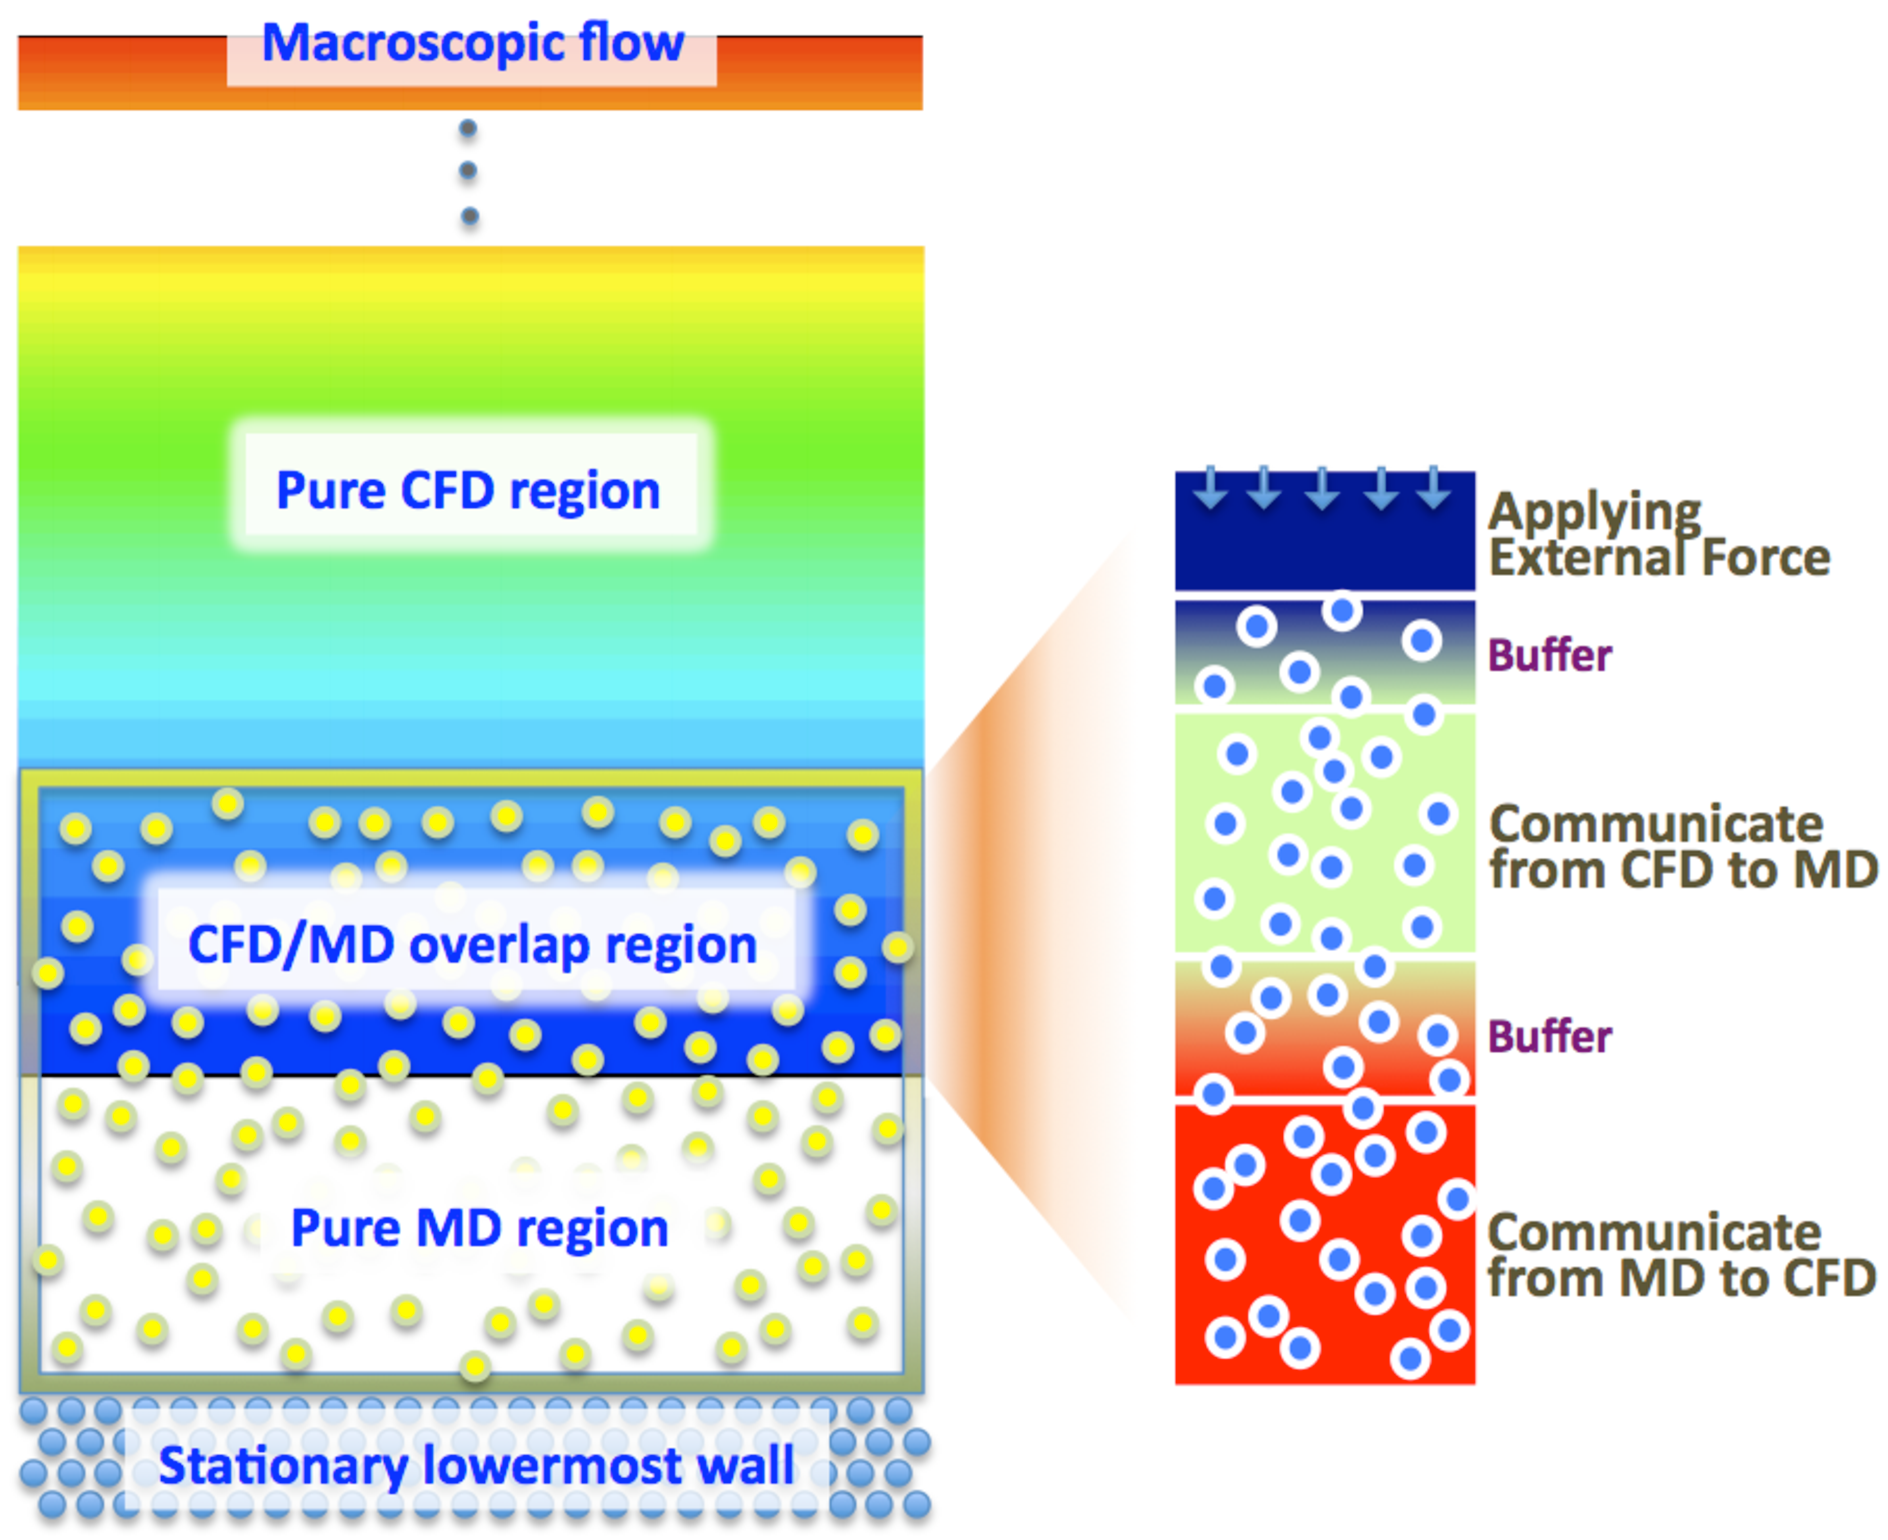
\includegraphics{Hybrid_Schematic.pdf}
%\caption{Schematic Diagram of the Hybrid Domain with Detailed View of Overlapping Zone: 
%Left figure expresses the composition of hybrid simulation domain and 
%the right figure presents individual layers in the overlapping region.}
%\end{wrapfigure}
\begin{figure}
\centering
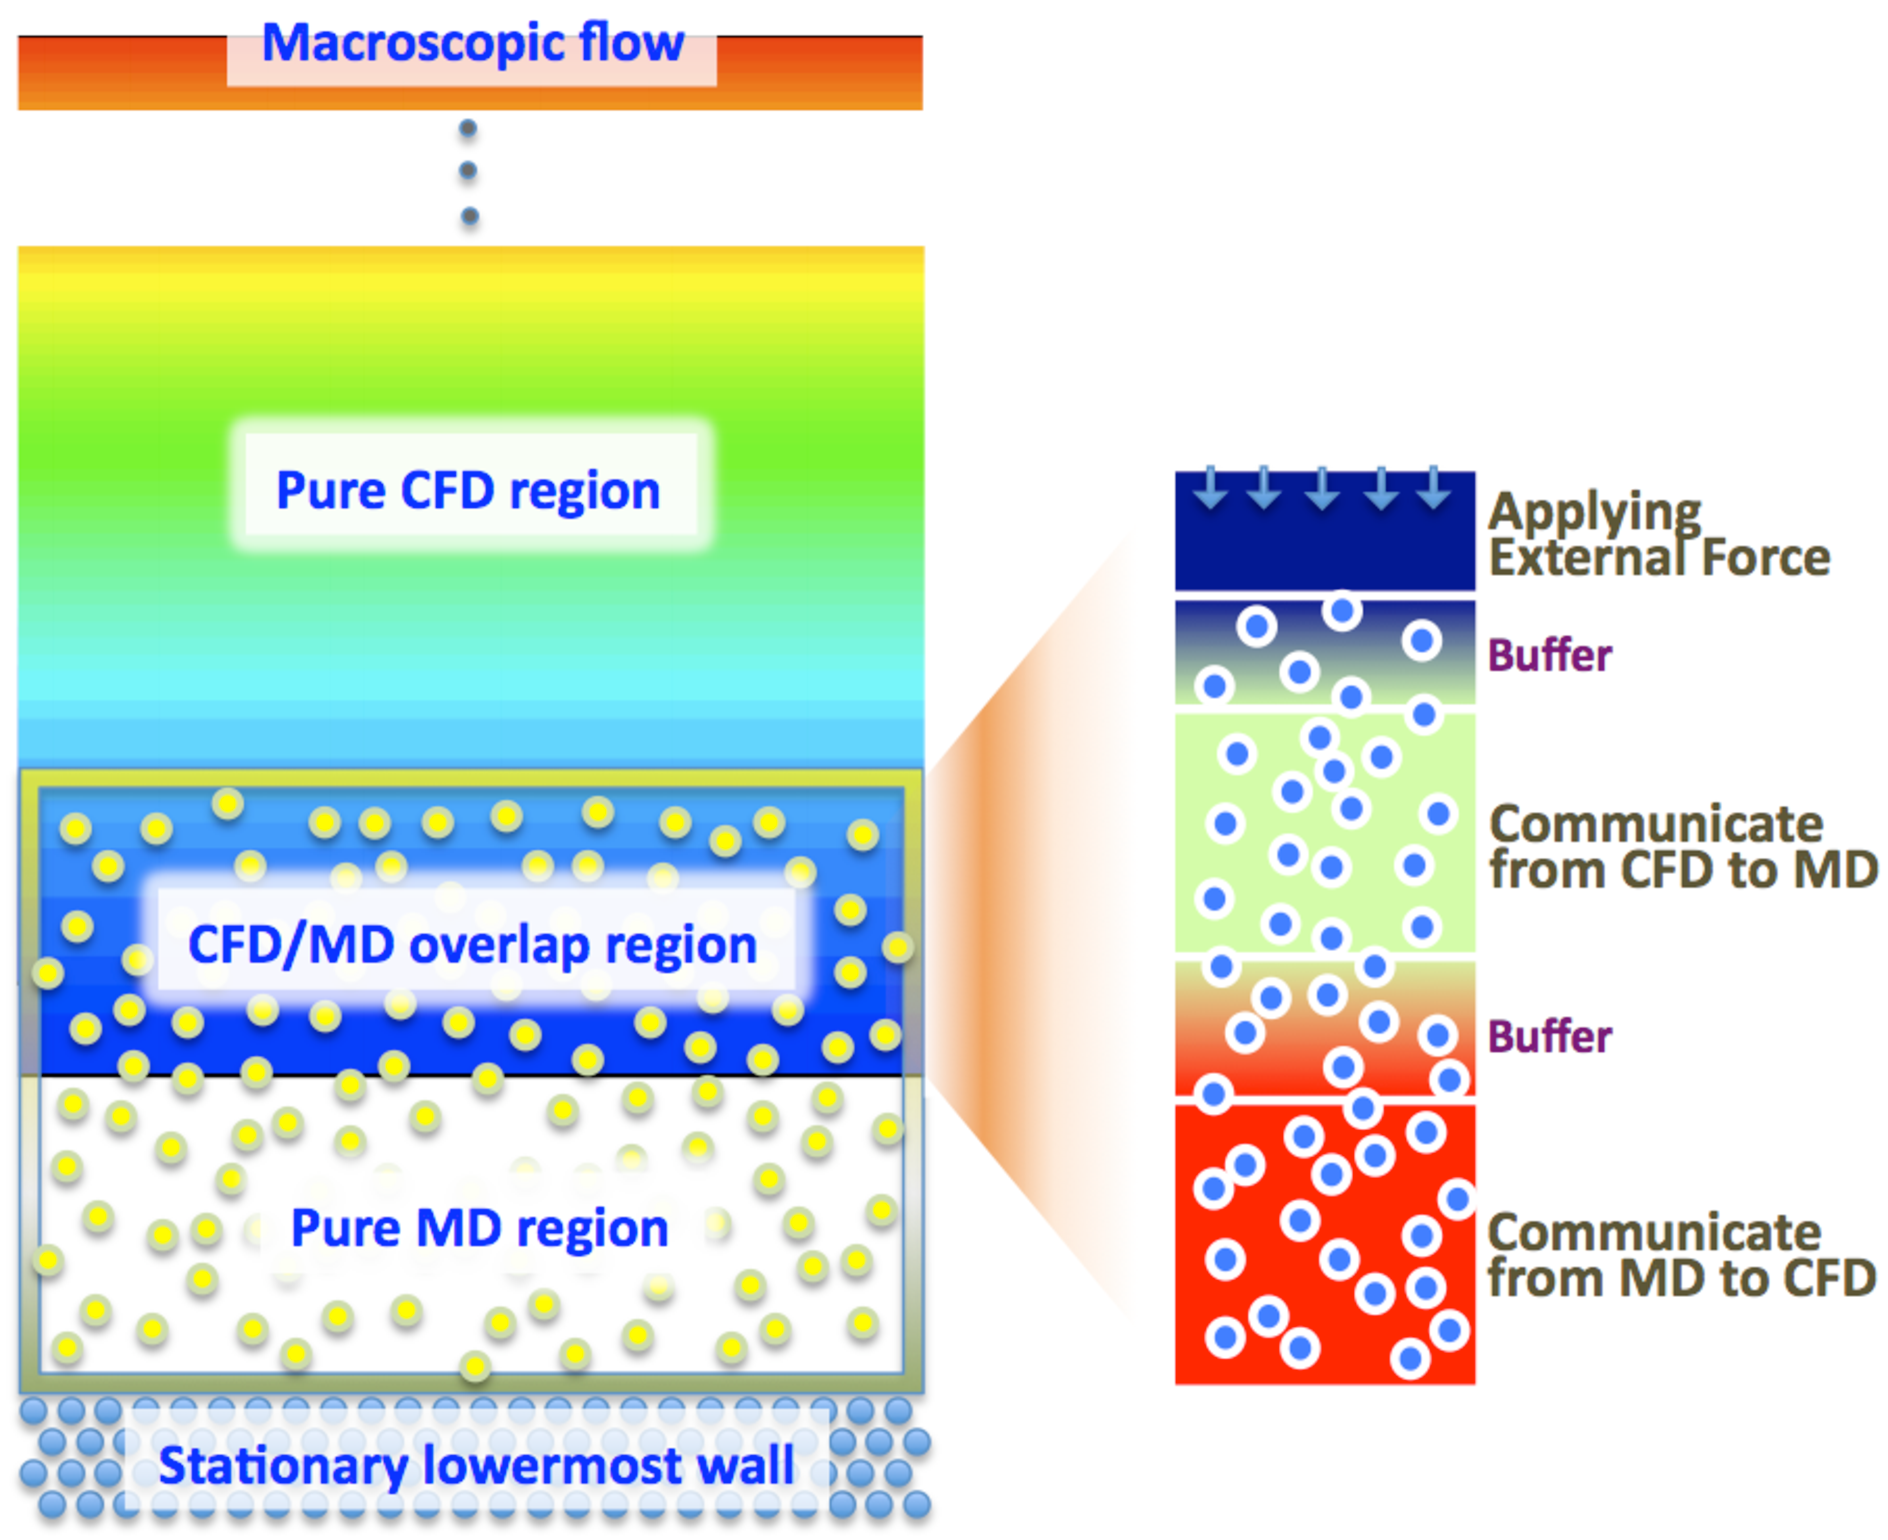
\includegraphics[width=0.6\linewidth]{Hybrid_Schematic.pdf}
\caption{Schematic Diagram of the Hybrid Domain with Detailed View of Overlapping Zone: 
Left figure expresses the composition of hybrid simulation domain and 
the right figure presents individual layers in the overlapping region.}
\label{Fig:Couette}
\end{figure}
%%%%% FIGURE %%%%%


The overlapping region is designed sufficiently large to contain 
five individual layers with sufficient spacing. From the bottom, 
we have the {\it{particle-to-continuum}} and {\it{continuum-to-particle}} 
(denoted as 'MDtoCFD' and 'CFDtoMD', respectively) layers where hybrid
boundary condition for CFD and MD are imposed. The external force layer
for particle systems is placed on the top (farthest from the
material interface) of the overlapping region. These three ''active'' layers 
are separated by the buffer layer, which is designed to prevent direct 
interaction between particles in above ''active'' layers.

Hybrid CFD boundary condition on MDtoCFD layer is imposed by averaging
molecular properties located in this layer. This boundary condition is prone to
suffer from the statistical error\cite{Hadjicon3,Time_Mechanism}, since
the finite number of particles participate in sampling process in space and time.
Therefore, the delicate determination of coupling parameters are very important
for acquiring the noise-free hybrid solution. The distance from the material 
interface and the size of sampling layer determines the scale of statistical 
error in space; how long the molecular properties will be accumulated
(''sampling duration'') and how often these samples are applied to the 
continuum solver (''sampling interval'') also affects the sampling noise in time.

The hybrid MD boundary condition is imposed by referencing the continuum solution
in this layer. A single set of continuum solution is imposed to higher
degree-of-freedom molecular domain through the constrained Lagrangian dynamics
equation. This equation constrains particles to attain the macroscopic flow property 
(conservative properties) on average, while preserving their degree-of-freedom of 
translational motion. Details on this equation will be presented in Section
\ref{sec:hybrid_multispecies}.

In the uppermost layer, a fictitious external force is exerted on particles 
to preserve the system ensembles of the particle domain. This force function
is designed to be short-range so as not to influence the motion of the particles 
past the buffer layer in the CFDtoMD domain. The force stiffens as the particles 
approach outer region to prevent the particles from drifting out of the 
particle domain. We apply a cost-effective classical external force model 
by Nie {\it{et al.}}\cite{Nie}. 


\subsection{Constrained Lagrangian Dynamics for Multi-species Fluid Simulation}
\label{sec:hybrid_multispecies}

\skonote{To Nayong: What shall be added here}

1. How classical constrained Lagrangian dynamics equation is implemented

-- what is the objective: to eventually equilibrate the continuum and mean microscopic velocity

-- what is the governing equation: the governing equation and the meaning of each term under the equation

2. Why it needs change

-- The limitation of the equation to be applied to multi-species fluid model

3. How it is improved

-- The formulation of "Polyatomic Multi-species Constrained Lagrangian Dynamics Equation"

-- Difference compared to the original equation

-- Difference in applying the equation: apply on the center of mass of each molecule, not on individual atom (which will imply that atoms under the same molecule will experience the same acceleration, which tells that the linear momentum is of particular concern)

%%%%% End Hybrid Schema %%%%%


%%%%% Numerical Schemes %%%%%
\section{Development of a Hybrid CFD-MD Simulation Package}
\label{sec:numerics}

We address the numerical schemes and hybrid interface of individual CFD and MD
solvers in brief: full details can be found in Ref.~\citen{JoCS2012}.

\subsection{Continuum Incompressible Flow Solver}
\label{sec:numerics_cfd}

The current in-house continuum hydrodynamics code solves the unsteady 
incompressible Navier-Stokes equations. In this work, the pseudo-compressibility 
method\cite{PseudoCompressibility} is adopted to form a hyperbolic system of 
equations which can be marched in pseudo-time.
For time-accurate unsteady simulation, a dual time stepping method is adopted 
and it is combined with the LU-SGS (Lower-Upper Symmetric Gauss-Seidel) scheme
\cite{LU-SGS} for the implicit time integration. The inviscid fluxes are 
upwind-differenced using Osher's flux-difference splitting scheme\cite{Osher}. 
For higher-order spatial accuracy, the MUSCL (Monotone Upstream-centered 
Schemes for Conservation Laws)\cite{MUSCL} approach is used on the inviscid 
flux calculation. Viscous fluxes are calculated using conventional 
second-order central differencing.


%The current in-house continuum hydrodynamics code solves the unsteady 
%incompressible Navier-Stokes equations: 

%\vspace{-.2em}
%\begin{eqnarray}
%\frac{\partial {u}_{i}}{\partial {x}_{i}} = 0
%\end{eqnarray}
%\vskip-.6cm
%\begin{eqnarray}
%\frac{\partial {u}_{i}}{\partial t} + \frac {\partial} {\partial {x}_{j}} ({u}_{i}{u}_{j}) = -\frac {\partial p} {\partial {x}_{i}} + \nu \frac {{\partial}^2 {u}_{i}} {{\partial} {x}_{j} \partial {x}_{j}} \nonumber
%\end{eqnarray}
%where $\nu$ is the kinematic viscosity.

%In this work, the pseudo-compressibility method\cite{PseudoCompressibility} 
%is adopted to form a hyperbolic system of equations which can be marched 
%in pseudo-time.
%A time derivative of pressure is added to the continuity equation resulting in

%\vspace{-.2em}
%\begin{eqnarray}
%\frac{\partial (p/\rho)}{\partial \tau} = - \beta \frac{\partial {u}_{i}}{\partial {x}_{i}}
%\end{eqnarray}
%where $\beta$ denotes a pseudo-compressibility parameter, currently set up to 2.5.

%For time-accurate unsteady simulation, a dual time stepping method is adopted 
%and it is combined with the LU-SGS (Lower-Upper Symmetric Gauss-Seidel) scheme
%\cite{LU-SGS} for the implicit time integration. The inviscid fluxes are 
%upwind-differenced using Osher's flux-difference splitting scheme\cite{Osher}. 
%For higher-order spatial accuracy, the MUSCL (Monotone Upstream-centered 
%Schemes for Conservation Laws)\cite{MUSCL} approach is used on the inviscid 
%flux calculation. Viscous fluxes are calculated using conventional 
%second-order central differencing.


\subsection{Particle Dynamics Solver}
\label{sec:numerics_md}

Newton's conservation of momentum is employed at the atomic level to propagate 
the system's motion through time evolution. In this work the most commonly used 
Lennard-Jones (12-6) intermolecular force potential model\cite{Allen} is employed 
to calculate pair-wise interactions of particles in the system. A cut-off distance
is introduced to reduce the computational cost and is set to be 2.2 magnitude of
atomic characteristic length\cite{Travis}. The most common velocity Verlet 
algorithm\cite{Allen} is employed for time integration of the equations of motion 
of the interacting particles and to compute molecular trajectories in the simulation.
In this work, the MD simulations were performed by using an appropriately 
modified version of the Large Atomic Molecular Massively Parallel Simulator 
(LAMMPS). It is a classical molecular dynamics open-source code written in C++ 
and developed by Sandia National Labs\cite{LAMMPS_url}.

%In MD, an initial velocity is assigned to each atom, and Newton's conservation 
%of momentum is employed at the atomic level to propagate the system's motion 
%through time evolution. In this work the most commonly used Lennard-Jones 
%(12-6) intermolecular force potential model is employed to calculate pair-wise 
%interactions of particles in the system, and is defined as:

%\vspace{-.2em}
%\begin{equation}
% u(|r_{i} - r_{j}|) = 4\epsilon_{ij}[(\frac{\sigma_{ij}}{r_{ij}})^{12}-(\frac{\sigma_{ij}}{r_{ij}})^{6}]
% \label{eq:LJ12}
%\end{equation}
%\normalsize

%where  $\epsilon_{ij}$ and $\sigma_{ij}$ denote the pair-wise potential well 
%depth and the atom size parameter respectively, and rij is the distance between 
%the particle i and j. The repulsive term $\it 1/r_{ij}^{12}$ dominating at 
%short $r_{ij}$ distance is based on the Pauli principle to avoid 
%overlapping the electronic clouds when particles are very close to each other. 
%The attractive term $\it 1/r_{ij}^{6}$ dominates at long range representing 
%Van der Waals dispersion forces. A cut-off distance $\sigma_{c}$ is introduced 
%here to reduce the computational cost and is set to be 2.2$\sigma$\cite{Travis}.
%Namely when $r_{ij}$ exceeds the cutoff the intermolecular force is set to zero 
%without being calculated.

%The most common velocity Verlet algorithm is employed for time integration 
%of the equations of motion of the interacting particles and to compute molecular 
%trajectories in the simulation.

%In this work, the MD simulations were performed by using an appropriately 
%modified version of the Large Atomic Molecular Massively Parallel Simulator 
%(LAMMPS). It is a classical molecular dynamics open-source code written in C++ 
%and developed by Sandia National Labs~\cite{LAMMPS_url}.


\subsection{Implementation of Hybrid Schemes and Interface}
\label{sec:numerics_hybrid}


The file-based communicator is implemented on each solver to exchange conservative
properties at every sampling interval. CFD solver stores the instataneous solution
at that time instance, while MD solver produces the backward sample over the
sampling duration. Thus, the extrapolation/interpolation mechanism for time-accurate
hybrid simulation\cite{JoCS2012} is also incorporated to avoid time-lagging pattern. 
CFD solver directly applies these extrapolated/interpolated properties as the 
hybrid boundary condition. MD solver inputs these values on employed constrained 
Lagrangian dynamics formulation. MD solver also applies the external force function
in the uppermost layer.

The unit conversion function is also incorporated in CFD solver. This function changes
the CFD non-dimensional solution into MD non-dimensional unit and vice versa. 
Considering the current formulation of CFD solver, the artificial pressure property
needs to be converted to an equivalent molecular mass density. The artificial pressure
is converted as,

(Equation to be implemented)

Coupling parameters, such as location and size of hybrid layers in space and 
sampling interval and sampling duration in time, are delicately determined 
by the reference to previous studies\cite{Nie,Yen,Liu,Hadjicon2,Werder,Flekkoy,Delgado1}
and preliminary measurement of noise level on pure molecular dynamic domain.
We also apply the replica sampling approach\cite{REMD} in case the individual 
hybrid solution suffers from the excessive sampling noise. This approach averages 
multiple independent simulations from the different initial Maxwell-Boltzmann 
distribution to find the non-fluctuating solution. The solution from N replicas 
provide the same order of accuracy as an individual solution from N times larger 
domain: this approach (running multiple small tasks instead of one big task) is 
computationally more effective in view of scheduling on many supercomputing
resources.


%%%%% Conclusion and Future Works %%%%%
\section{Conclusion and Future Works}
\label{sec:conclusion}


Accurate and efficient multi-scale flow simulations by a hybrid CFD-MD simulation framework have been presented in this paper. Constrained Lagrangian dynamics equations of motion and file-based hybrid interfaces are implemented on a highly-reliable LAMMPS molecular dynamics package and a verified in-house incompressible CFD code. They are virtually integrated as a single BigJob framework.

A number of numerical issues which harm the accuracy of a hybrid solution have been explored. First, quantifying the sampling noise from a stationary flow has been proposed as a way of determining coupling parameters. We argue that our simple and intuitive idea unveils the influence of individual coupling parameter on the magnitude of statistical error and is very cost-effective in contrast to traditional trial-and-error approach.
%until getting a stable solution.
Moreover, the empirical equation derived from the stationary flow simulation describes that well-know mathematical expressions on statistical error are not accurate on nano-scale wall-bounded systems.
Second, sampling multiple independent replicas has been introduced to refine the sampling noise of an individual solution and to explore to the low-speed flow regimes. This approach is superior to simulating a single large-scale problem set which is technically bound by computing capacity. The application to a Couette flow simulation in O(10) m/s velocity field is the first successful report of a moderate-speed flow simulation using a hybrid CFD-MD approach.
Last, a prediction-correction approach has been designed for the accurate unsteady simulation. This approach acquires better solution by enabling the imposition of interpolated hybrid boundary conditions. The application to the oscillating boundary problem expresses that the current approach diminishes the overshoot/undershoot phenomena in the conventional methods.

Along with numerical issues, computational issues for the efficient coupled simulations have been also discussed. We introduced a BigJob framework and this directly solves the co-scheduling problem among logically separated sub-tasks. A simple load-balancing function is also implemented on a BigJob framework, to achieve the load-balancing among those separated-yet-coupled codes. From numerical experiments, we evaluate that a BigJob is very powerful in reducing the waiting time of the coupled simulation. Also, a simple load-balancing function employed in a BigJob is effective in reducing the simulation runtime.

We emphasize that above numerical investigations ease the challenge to the hybrid simulation and broaden the application area. Also, our computational experiments contribute on how to efficiently conduct coupled simulations.



%The empirical mathematical equation on sampling noise has been presented in Sec.~\ref{sec:accuracy_conditions}. We argue that this is a refined model compared to previous mathematical expressions. However, the formulation has not been verified by various systems and conditions: coefficients will be changing according to the distance from the wall, characteristics of fluid and solid elements, etc. More rigorous research is required to address a globally acceptable equation of sampling noise.

Numerical simulations in Sec.~\ref{sec:accuracy} demonstrates that the delicate determination of coupling parameters along with the supplementary use of replica sampling approaches (in Sec.~\ref{sec:numerical_noise} is very important for the accurate hybrid simulations. Unfortunately, coupling conditions have been rather intuitively or empirically determined according to the flow physics of the target problem, and proposed mathematical expressions in statistical error~\cite{Hadjicon3,Time_Mechanism} fails to consider the variation of sampling noise depending on the geometric configuration. It is highly required to develop a mathematical model for predicting the sampling noise in wall-bounded flow systems.

Unsteady flow simulation in Sec.~\ref{sec:accuracy_oscillation} verifies that the prediction-correction approach provides more accurate solution than conventional temporal coupling scheme. The new approach is especially powerful in resolving the unfavorable overshoot/undershoot phenomena. On the other hand, the slight time-lagging effect in the conventional model has not been improved by the prediction-correction approach. We expect that this phenomenon can be resolved by applying higher-order extrapolation/interpolation on hybrid boundary regions.

%The unstable solution at Fig.~\ref{Couette_Noisy} represents the result of Couette flow simulation with 0.1 $\sigma / \tau$ upper plate velocity in O(100) nanometer system. The diverging solution is intuitively natural, according to the statistical noise measurement in Table~\ref{table:MD_Vel0_L}: the amount of statistical error is 25 percent of the steady-state velocity in MDtoCFD layer. For the worse, the signal-to-noise ratio is even larger at early stage. Thus the strong initial instability makes it harder for the solver to reach the steady-state solution. Increasing the sampling duration to 1000 $\tau$ did not help; increasing the height of layers implies the abandonment of hybrid method's merit over pure MD method.
%Clearly, this is one of the most important issues to make the family of hybrid methods a powerful tool which describes the detailed phenomena between solid obstacles and surrounding fluids more accurately. So far, two possible ways are observed at the first glance. First, setting the initial MD condition the same as steady-state CFD profile and starting hybrid simulation will, at least, alleviate the influence of noise at early stage. However, time-accurate unsteady solution can not be gained by this approach. Second, \skonote{check the clear term of zeta at Nie's formulation!} increasing $\zeta$ looks helpful in alleviating the noise in system level. However, this is worried whether excessive suppress of particles' vibration results in the breakup of fluid physics, i.e., breakup of energy conservation. A thorough investigation on the characteristics of statistical noise and design of numerical algorithm for acquiring the accurate solution without numerical damping are highly required.

%%\begin{figure}[ht!]
%\begin{figure}
%\centering
%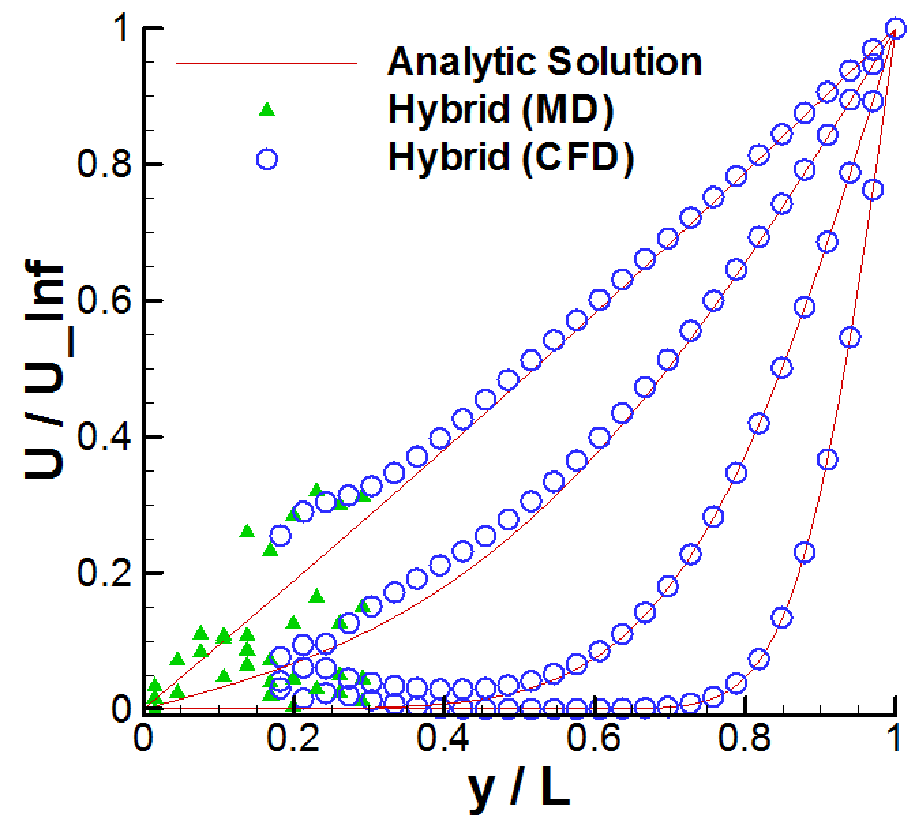
\includegraphics[width=0.6\linewidth]{Couette_Noisy.pdf}
%\vskip-0.2cm
%\caption{\small {\bf Unstable solution at low shear rate.} Velocity of the upper plate is 0.1 $\sigma / \tau$ and all other conditions are identical to the Couette flow simulation in large domain. The solution diverges at early stage, since the statistical error is very large compared to the hydrodynamic velocity.}
%\label{Stokes_Sol}
%\end{figure}



%%%%% End Conclusion and Future Works %%%%%


%%%%% Acknowledgement %%%%%
\section*{Acknowledgement}

Content

%%%%% End Acknowledgement %%%%%


% produces the bibliography section when processed by BibTeX
\bibliography{Bibs/Hybrid}
\bibliographystyle{aiaa}

\end{document}

% - Release $Name:  $ -
